% TMLR submission (anonymised). Build: tectonic main.tex   (or latexmk -pdf main.tex)
% Uses the official TMLR style (tmlr.sty, tmlr.bst from github.com/JmlrOrg/tmlr-style-file) when present in this
% folder; otherwise falls back to article + natbib so the draft still compiles.
\documentclass[10pt]{article}

\IfFileExists{tmlr.sty}{%
  \usepackage{tmlr}            % anonymous submission; use [accepted] or [preprint] later
  \newcommand{\bibstylename}{tmlr}%
}{%
  \usepackage[margin=1in]{geometry}
  \usepackage[round]{natbib}
  \newcommand{\name}[1]{##1}\newcommand{\addr}[1]{\\ ##1}
  \newcommand{\bibstylename}{plainnat}%
}

\usepackage{amsmath,amssymb}
\usepackage{booktabs}
\usepackage{graphicx}
\usepackage{xcolor}
\usepackage{enumitem}
\usepackage{hyperref}
\usepackage{url}
\graphicspath{{../../results/figures/}}

\newcommand{\aopt}{\alpha_0^{\star}}
\newcommand{\qeff}{q_{\mathrm{eff}}}
\newcommand{\best}[1]{\textbf{#1}}

\title{Scaling Laws for Stochastic-Approximation EM:\\ One Recipe and One Step-Size Rule across Five Model Families}

\author{\name Anonymous authors \addr Paper under double-blind review}

\IfFileExists{tmlr.sty}{%
  \def\month{MM}%
  \def\year{YYYY}%
  \def\openreview{\url{https://openreview.net/forum?id=XXXX}}%
}{\date{}}

\begin{document}
\maketitle

\begin{abstract}
e-means trains $k$-means with an exponential moving average (EMA) of each cluster's sufficient statistics, a
cosine-annealed rate, revival of dead clusters, and a fitted law that sets the initial rate from the problem size.
The update is stochastic-approximation (stepwise) EM, so it applies to any model with a closed-form M-step. We test
the full recipe on Gaussian mixtures, hidden Markov models, latent Dirichlet allocation, online dictionary learning /
NMF and alternating least squares: 19 dataset configurations, 5 seeds, budgets from 0.25 to 25 epochs, against
full-batch EM at 25 iterations and against stepwise EM tuned on the same validation grid. With its rate selected on
validation, the recipe reaches the batch objective in under 3 epochs on 12 of 19 configurations (median 38$\times$
fewer epochs on HMMs, 30$\times$ on dictionary learning). Against tuned stepwise EM given the same revival rule, it
reaches the batch objective sooner on 16 of 19 configurations and is never significantly worse outside LDA. An
ablation separates the components: revival is what makes stochastic EM work where components die (full-covariance
GMMs, LDA), and the cosine schedule is what beats tuned step decay where they do not (HMMs, dictionary learning).
Matched-quality CPU wall-clock speed-ups reach 5--82$\times$. The $k$-means rate law, applied unchanged, transfers to
four families (median validation penalty $\le 0.2\%$) but fails on LDA, whose optimal rate is about an order of
magnitude lower. A pre-registered cross-family law beats per-family constants (leave-one-cell-out median penalty
0.11\% vs 0.32\%), and re-expressing it in observations per sufficient-statistic cell explains two-thirds of the
variance of the optimal rate with one global fit and cuts the held-out penalty on LDA from 28\% to 12\%
(exploratory). Code and all 44{,}197 run records are released.
\end{abstract}

%======================================================================================================================
\section{Introduction}

Expectation--maximisation (EM) for latent-variable models with exponential-family complete-data likelihoods touches
the data only through expected sufficient statistics. Replacing the full-data average of those statistics with a
running, step-size-weighted average over mini-batches gives stochastic-approximation EM. The method has several
names and origins: online EM \citep{sato2000online,cappe2009online}, stepwise EM \citep{liang2009online}, and the
natural-gradient step of stochastic variational inference \citep{hoffman2013svi}. It is a standard tool for single
families: online LDA \citep{hoffman2010online}, online dictionary learning \citep{mairal2010online} and mini-batch EM
for mixtures \citep{nguyen2020minibatch}. In practice its step-size schedule is tuned per problem;
\citet{liang2009online} already noted that the best schedule depends on the task and dataset.

e-means \citep{bessa2026emeans} revisited this update for $k$-means at billion scale. It adds three ingredients:
\begin{itemize}[nosep]
  \item a \emph{cosine-annealed} rate in place of the usual inverse-time decay $(\tau_0 + t)^{-\kappa}$;
  \item a \emph{revival} rule that re-seeds clusters whose EMA mass collapses;
  \item a \emph{scaling law} that predicts the initial rate $\alpha_0$ and the batch size from $(n, k, B, T)$, fitted on
        one dataset.
\end{itemize}
It reports reaching Lloyd's objective in about a tenth of the epochs. The paper calls its update a hard-assignment
form of EM with decayed statistics but tests no other model.

This paper asks whether that recipe, including its law, is a property of stochastic-approximation EM in general or
of $k$-means. We answer with a pre-registered, cross-family study:
\begin{enumerate}[nosep]
  \item \textbf{The recipe transfers (C1).} On 12 of 19 configurations across five families, the recipe with
        $\alpha_0$ selected on validation reaches full-batch EM@25 in $\le 3$ epochs. Where it does not
        (full-covariance GMMs on real data, two LDA corpora, ALS), we report how long it takes.
  \item \textbf{Against the strongest baseline, the schedule matters except on LDA (C2, C2b).} We compare with
        stepwise EM tuned on the same grid \emph{and given the same revival rule}. The recipe is significantly better
        on 51 of 102 (configuration, budget) cells, tied on 47 and worse on 4, all on LDA. The ablation separates the
        components: revival rescues stochastic EM on full-covariance GMMs (SIFT1M: 50.7 $\to$ 40.5 nats against a
        batch reference of 40.7) and LDA. The schedule is the whole advantage on HMMs (up to 10\% lower held-out NLL
        at one epoch) and dictionary learning.
  \item \textbf{Wall-clock (C3).} In an isolated CPU timing pass, matched-quality speed-ups over batch EM@25 are
        5.4--82$\times$ for every configuration that matches within 5 epochs.
  \item \textbf{The $k$-means law transfers, except to LDA (C4).} Unchanged, it costs $\le 0.2\%$ median validation
        loss on GMM, HMM, dictionary learning and ALS. On LDA it never reaches the batch reference.
  \item \textbf{A cross-family law (C5, pre-registered) and a coordinate that explains the LDA anomaly (C6,
        exploratory).} One law with per-family constants beats per-family constants alone. Written in observations
        per sufficient-statistic cell per step, a single global law explains 66\% of the variance of $\log\aopt$
        (vs 20\% in the $k$-means coordinates) and shrinks the LDA held-out penalty from 28\% to 12\%. It is not
        universal: the exponent on observations per cell is 0.43, not 1, and HMMs want the maximum rate despite
        sparse cells.
\end{enumerate}
We frame the contribution as an empirical and predictive study of stochastic-approximation EM at scale. We make no
claim to a new update rule: the update is stepwise EM, and tuned stepwise EM is our main baseline throughout.

%======================================================================================================================
\section{Related work}

\paragraph{Online / stepwise EM and SVI.}
Incremental EM \citep{neal1998view}; online EM for normalised Gaussian networks \citep{sato2000online}; convergence
of online EM with Robbins--Monro steps \citep{robbins1951stochastic,cappe2009online} and of SAEM
\citep{delyon1999saem}; stepwise EM on four NLP models, 2--10$\times$ faster than batch EM with a task-dependent step
\citep{liang2009online}; online LDA and SVI \citep{hoffman2010online,hoffman2013svi}; online dictionary learning
and NMF \citep{mairal2010online}; and mini-batch EM for exponential-family mixtures, which lists step and batch
tuning as future work \citep{nguyen2020minibatch}. Our update is theirs. We differ in four ways: the schedule
(cosine instead of inverse-time), the revival rule, a time-to-batch protocol across five families, and a fitted law
for the rate.

\paragraph{Step-size adaptation.}
\citet{ranganath2013adaptive} remove tuning for SVI by estimating the step online; we instead predict the initial
rate from problem coordinates. Variance-reduced stochastic EM \citep{chen2018sem} uses a constant step with control
variates and is complementary. Riemannian batch and stochastic optimisation \citep{hosseini2020alternative} is an
alternative to EM-style updates for GMMs.

\paragraph{Dead components.}
\citet{sato2000online} already add unit production, deletion and division to online EM, to track changing
environments. Memoized online VI with birth/merge moves \citep{hughes2013memoized} is the closest modern mechanism.
$k$-means codebooks commonly re-seed empty clusters \citep{johnson2019faiss,douze2024faiss}, and e-means uses a donor
split. \citet{weiss2026small} refine e-means' count-based rule for $k$-means: a small cluster is removed only if it is
close to another centre, which protects rare isolated groups (we test this variant in Appendix~\ref{app:rare}). We
know of no single dead-component rule applied across EM families.

\paragraph{Scaling laws and hyperparameter transfer.}
Empirical laws for learning rate and batch size in neural network training are well established: the gradient noise
scale \citep{mccandlish2018empirical}, loss scaling laws \citep{kaplan2020scaling}, and fitted learning-rate and
batch-size laws \citep{deepseek2024llm}. \citet{busbridge2023ema} show how to scale an EMA with batch size. The cosine
schedule comes from SGD \citep{loshchilov2017sgdr}. e-means fitted such a law for $k$-means on one dataset. We test
whether it transfers across families, and in which coordinates.

\paragraph{Fast exact kernels.}
Flash-KMeans \citep{yang2026flashkmeans} and Flash-GMM \citep{bloch2026flashgmm} are fused GPU kernels that make each
exact Lloyd or EM iteration cheaper without storing the $N \times K$ distance or responsibility matrix. They change
the cost per pass, not the number of passes, and would apply equally to the mini-batch E-step of the recipe. They are
therefore complementary to this paper, which counts passes and reports wall-clock only from a like-for-like CPU
implementation of both sides.

%======================================================================================================================
\section{Method}

\subsection{Stochastic-approximation EM with EMA statistics}
Let the complete-data model be in the exponential family with sufficient statistics $s(x, z)$. Batch EM alternates
an E-step, $S = \frac{1}{n}\sum_i \mathbb{E}[s(x_i, z_i) \mid \theta]$, with a closed-form M-step $\theta = m(S)$.
The recipe keeps a running estimate $\hat S$ and, for each mini-batch $b_t$ of size $B$, sets
\begin{equation}
  \hat S_t = (1 - \alpha_t)\, \hat S_{t-1} + \alpha_t \cdot \frac{1}{B}\sum_{i \in b_t}
  \mathbb{E}[s(x_i, z_i) \mid \theta_{t-1}], \qquad \theta_t = m(\hat S_t).
\end{equation}
With $\alpha_t = (\tau_0 + t)^{-\kappa}$ this is stepwise EM; the tuned baseline uses this form. Table~\ref{tab:stats}
lists the statistics per family. For dictionary learning the M-step is a few passes of block-coordinate descent on
the dictionary columns given the EMA $(A, B)$, with a non-negativity projection for NMF \citep{mairal2010online}.

\begin{table}[t]
\centering\small
\caption{EMA statistics and M-step per family.}\label{tab:stats}
\begin{tabular}{p{2.6cm}p{6.6cm}p{4.6cm}}
\toprule
family & EMA statistics & M-step \\
\midrule
GMM (diag / full) & $N_j$, $\sum r_{ij} x_i$, $\sum r_{ij} x_i x_i^\top$ (or diagonal) & weights, means, covariances (+ ridge) \\
HMM & expected initial, transition, emission counts (forward--backward) & row-normalise \\
LDA & expected topic--word counts scaled by $D/B$ (SVI's global step) & $\lambda = \eta + \hat S$ \\
Dict.\ learning / NMF & $A = \sum \alpha\alpha^\top$, $B = \sum x \alpha^\top$ & block-coordinate dictionary update \\
ALS & per-item $n_i$, $b_i = \sum r u$, $A_i = \sum u u^\top$ & item factors from normal equations \\
\bottomrule
\end{tabular}
\end{table}

\subsection{Cosine schedule}
\begin{equation}
  \alpha_t = \alpha_0 \cdot \Big(\varepsilon + (1 - \varepsilon)\cdot \tfrac12\big(1 + \cos(\pi t / M)\big)\Big),
  \qquad \varepsilon = 0.1,
\end{equation}
where $M$ is the total number of steps in the budget $T$ (in epochs). The baseline schedule decays with $t$ regardless
of the budget. The cosine schedule ties the decay to the budget, keeping the rate high for most of the run and
annealing to $\varepsilon\alpha_0$ at the end.

\subsection{Revival}
Every 5 batches, any unit (mixture component, topic, state, dictionary atom) with EMA mass $N_j < 0.1 \cdot
\mathrm{mean}(N)$ is re-seeded by splitting a live donor drawn with probability proportional to its mass: the donor's
statistics are shared and slightly perturbed, as in e-means. One implementation serves all families. Families without
per-component mass (ALS) do not use revival. Statistics start at $N = 10^{-10}$, so the first batch effectively
initialises them.

\subsection{Rate laws}
\begin{itemize}[nosep]
  \item \textbf{$k$-means law (e-means, unchanged):} $\alpha_0 = \min(0.824\, k^{-0.46} B^{0.90} n^{-0.45}
        T^{-0.11}, 1)$, with $B$ from the e-means batch law. We call the recipe with this $\alpha_0$ the \emph{law}
        method (untuned).
  \item \textbf{Cross-family law M1 (pre-registered):} $\log\aopt$ linear in $\log(n/k)$, $\log B$ and $\log T$ with
        per-family intercepts, fitted on swept optima across all families. The null M0 is per-family constants only.
  \item \textbf{Per-cell coordinates (exploratory):} $q$ = observations reaching each sufficient-statistic cell per
        step: $B/k$ for GMMs; $B \times$ code density for dictionary learning; $B \times$ (ratings per user) / items
        for ALS; $B \times$ (tokens per document or sequence) / $(KV)$ for LDA and HMMs. $\qeff$ replaces $V$ with the
        effective vocabulary $\exp(H(\text{unigram}))$. The global law is
        $\log\aopt = c + a\log\qeff + b\log(n/B) + d\log T$.
\end{itemize}

%======================================================================================================================
\section{Experimental protocol}

\paragraph{Families and data (19 configurations).} Table~\ref{tab:data}. Dataset sources, licences and preprocessing
are in Appendix~\ref{app:data}.

\begin{table}[t]
\centering\small
\caption{Families, data and references.}\label{tab:data}
\begin{tabular}{p{2.1cm}p{5.6cm}p{1.6cm}p{2.0cm}p{1.9cm}}
\toprule
family & datasets (configurations) & $k$ & test metric & reference \\
\midrule
GMM & synthetic, SIFT1M-PCA64, DINOv2-PCA64, AG News-PCA64 (MiniLM); diag and full covariance (8) & 32 / 64 & NLL / point & EM, 25 it. \\
Dict.\ learning / NMF & CIFAR $8{\times}8$ and $12{\times}12$ patches, 20 Newsgroups NMF (3) & 128 / 192 / 32 & recon.\ $+ \lambda\|\alpha\|_1$ & batch DL, 25 it. \\
LDA & 20 Newsgroups, Enron, NYTimes (UCI bag-of-words) (3) & 50 & held-out perplexity & batch VB, 25 it. \\
ALS & MovieLens 1M, 10M (2) & rank 32 & test RMSE & ALS-WR, 25 it. \\
HMM & synthetic, Brown POS, UCI HAR (vector-quantised) (3) & 12 & NLL / token & Baum--Welch, 25 it. \\
\bottomrule
\end{tabular}
\end{table}

\paragraph{Budgets and seeds.} Budgets $T \in \{0.25, 0.5, 1, 2, 3, 5, 10, 25\}$ epochs; seeds 0--4 for every method
and configuration. Train / validation / test splits are fixed per seed.

\paragraph{Methods.}
\begin{itemize}[nosep]
  \item \emph{swept} (ours): $\alpha_0$ selected on validation per budget from an 8-point log grid on $[0.01, 1]$. The
        LDA grid is extended below 0.01 where the optimum sat at the floor.
  \item \emph{law} (ours, untuned): the $k$-means law.
  \item \emph{tuned stepwise / online EM} (published prior art): $(\tau_0, \kappa)$ from an 18--24-point grid,
        selected on the same validation protocol, without revival.
  \item \emph{tuned stepwise + revival} (ablation): the same grid and selection plus our revival rule.
  \item Library defaults as sanity checks: scikit-learn GaussianMixture and MiniBatchDictionaryLearning
        \citep{pedregosa2011sklearn}, hmmlearn \citep{hmmlearn}, and the online-LDA defaults of
        \citet{hoffman2010online}.
\end{itemize}

\paragraph{Long budgets.} At $T = 10$ and 25 both our method and the baselines search a frozen 3--4-point
neighbourhood of their own $T = 5$ optimum. This was fixed before any long run.

\paragraph{Metrics.}
\emph{Epochs-to-match} is the first, linearly interpolated, epoch at which the seed-mean test curve reaches the
seed-mean reference@25; gain $= 25 /$ epochs-to-match. We report 95\% CIs by seed bootstrap and paired $t$-tests by
seed ($\alpha = 0.05$). The \emph{law penalty} is the relative validation loss of the predicted $\alpha_0$ against
the swept optimum, scored leave-one-cell-out (LOCO) and leave-one-family-out (LOAO).

\paragraph{Pre-registration.} Hypotheses, kill criteria and the cross-family law test were frozen before the runs
(amendments logged in the released code). The revival-equipped baseline and the per-cell refit were added after
seeing results and are labelled as ablation and exploratory.

\paragraph{Hardware.} One desktop (Ryzen 9 9900X, RTX 5090). GPU ports of the hot loops are float64 and
parity-tested; they change wall-clock only. Headline wall-clock comes from a separate isolated pass: CPU only, 12
threads, one job at a time, 3 seeds, after warm-up.

%======================================================================================================================
\section{Results}

\subsection{Time to the batch objective (C1)}

\begin{table}[t]
\centering\small
\caption{Epochs to reach full-batch EM@25 (seed means, 5 seeds; --- = not within 25 epochs). Best per row in bold.}
\label{tab:epochs}
\setlength{\tabcolsep}{4pt}
\begin{tabular}{lcccc}
\toprule
configuration & swept (ours) & law (ours, untuned) & tuned stepwise & tuned stepwise + revival \\
\midrule
GMM synthetic diag & \best{0.29} & 17.2 & --- & 3.94 \\
GMM synthetic full & \best{1.98} & 2.88 & --- & 23.0 \\
GMM SIFT1M diag & \best{0.88} & 0.97 & --- & 1.64 \\
GMM SIFT1M full & \best{7.24} & 14.8 & --- & 10.4 \\
GMM DINOv2 diag & \best{1.88} & 2.04 & --- & 11.8 \\
GMM DINOv2 full & \best{8.78} & 23.1 & --- & 9.01 \\
GMM AG News diag & 2.54 & \best{2.04} & --- & 4.49 \\
GMM AG News full & \best{9.63} & 12.0 & --- & 16.0 \\
\midrule
DL CIFAR $8{\times}8$ & \best{$\le$ 0.25} & 1.68 & 0.54 & 0.54 \\
DL CIFAR $12{\times}12$ & \best{0.83} & 2.83 & 1.66 & 1.66 \\
DL 20NG NMF & \best{2.32} & 2.36 & 3.70 & 3.70 \\
\midrule
LDA 20NG & 1.13 & --- & 1.60 & \best{0.89} \\
LDA Enron & \best{4.44} & --- & --- & 7.17 \\
LDA NYTimes & --- (3242) & --- & --- (3317) & --- (\best{3198}; ref.\ 3167) \\
\midrule
ALS ML-10M & \best{5.84} & 8.88 & 20.1 & n/a \\
ALS ML-1M & --- (tie: 0.8656 = ref.) & --- & --- & n/a \\
\midrule
HMM Brown POS & \best{0.64} & 0.95 & 1.33 & 1.33 \\
HMM synthetic & \best{0.66} & 1.44 & 1.95 & 1.95 \\
HMM UCI HAR & \best{1.72} & 2.21 & 5.70 & 6.73 \\
\bottomrule
\end{tabular}
\end{table}

The swept recipe reaches the reference within 3 epochs on 12 configurations (Table~\ref{tab:epochs}): all four
diagonal GMMs and synthetic full covariance; all three dictionary-learning configurations; LDA 20NG; and all three
HMMs. Full-covariance GMMs on real data take 7--10 epochs. LDA Enron takes 4.4 epochs; on NYTimes no online method
reaches batch VB@25 within 25 epochs. ALS ML-10M takes 5.8 epochs; on ML-1M every online method ends within 0.0005
RMSE of an already-converged ALS-WR (a tie, not a loss). DL CIFAR $8{\times}8$ matches at the first budget (0.25
epochs), so its gain is a floor.

\begin{figure}[t]
\centering
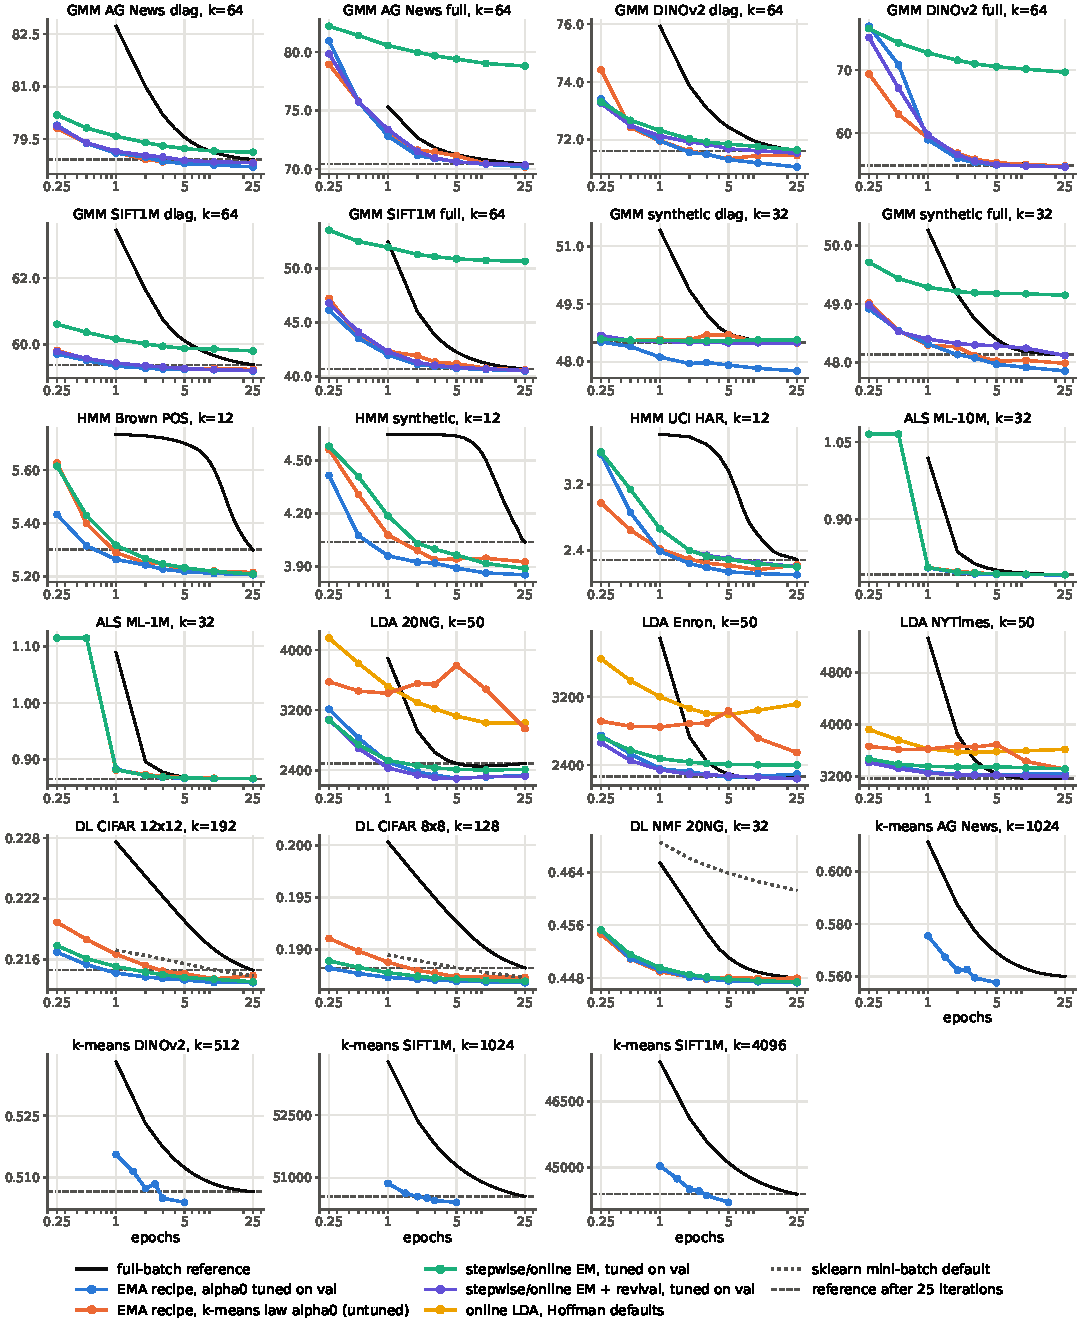
\includegraphics[width=\linewidth]{convergence.pdf}
\caption{Seed-mean test objective vs epochs (log scale) for every configuration. Black: full-batch reference; dashed:
the reference after 25 iterations.}
\label{fig:convergence}
\end{figure}

\subsection{Against tuned stepwise EM, and what the gain is made of (C2, C2b)}

The published stepwise / online EM baselines have no dead-component handling. Without it, full-covariance GMMs lose
most of their components: 57 of 64 die on SIFT1M. As a result, tuned online EM never reaches the batch reference on
any GMM configuration (SIFT1M full ends at 50.7 nats vs 40.7). Comparing our recipe only against this baseline would
credit the schedule with the effect of revival, so we add a baseline with the same $(\tau_0, \kappa)$ grid and
validation selection plus our revival rule.

\begin{table}[t]
\centering\small
\caption{Recipe (swept) vs tuned stepwise + revival, paired by seed at $T \in \{1, 2, 3, 5, 10, 25\}$. W / tie / L =
recipe significantly lower / no significant difference / significantly higher (two-sided paired $t$-test, 4 dof,
$p < 0.05$).}\label{tab:wtl}
\begin{tabular}{lcc}
\toprule
family (configurations) & W / tie / L & relative difference (recipe $-$ baseline) \\
\midrule
GMM (8) & 26 / 22 / 0 & $-0.03\%$ to $-1.5\%$ \\
HMM (3) & 14 / 4 / 0 & $-0.05\%$ to $-10.3\%$ \\
Dictionary learning (3) & 11 / 7 / 0 & $-0.03\%$ to $-0.30\%$ \\
LDA (3) & 0 / 14 / 4 & $-0.8\%$ to $+3.2\%$ \\
\bottomrule
\end{tabular}
\end{table}

\begin{table}[t]
\centering\small
\caption{Effect of revival on the tuned baseline (test objective at $T = 25$, seed means; lower is better).}
\label{tab:revival}
\begin{tabular}{lcccc}
\toprule
configuration & tuned stepwise & + revival & swept (ours) & reference@25 \\
\midrule
GMM SIFT1M full & 50.68 & 40.53 & 40.50 & 40.69 \\
GMM DINOv2 full & 69.64 & 54.61 & 54.65 & 54.80 \\
GMM AG News full & 78.81 & 70.37 & 70.20 & 70.42 \\
LDA 20NG & 2410 & 2320 & 2334 & 2489 \\
LDA Enron & 2401 & 2240 & 2295 & 2267 \\
LDA NYTimes & 3317 & 3198 & 3242 & 3167 \\
HMM / DL & \multicolumn{4}{c}{identical with and without revival (it never fires)} \\
\bottomrule
\end{tabular}
\end{table}

Three findings follow (Tables~\ref{tab:wtl} and~\ref{tab:revival}).
\begin{enumerate}[nosep]
  \item \textbf{Revival is what makes stochastic EM viable} where components can die. With it, the tuned baseline
        reaches the batch reference on all 8 GMM configurations. On LDA it lowers final perplexity on all three corpora
        and turns Enron from never matching into a match at 7.2 epochs.
  \item \textbf{With revival on both sides, the cosine schedule still helps on three of four families.} On GMMs the
        margin is modest (0.03--1.5\%); on real-data full covariance it is significant only at $T \le 2$ and ties
        afterwards. On HMMs it is large and persists to 25 epochs on UCI HAR ($-4.5\%$). On dictionary learning it is
        small but consistent.
  \item \textbf{On LDA, a tuned inverse-time schedule with revival is as good or better.} It matches the batch
        reference sooner on 20NG (0.89 vs 1.13 epochs) and ends lower on Enron and NYTimes at $T = 25$. The recipe's
        held-out perplexity rises from $T = 5$ to $T = 25$ on all three corpora (e.g.\ 20NG 2290 $\to$ 2334), and so
        does batch VB's (2456 at 10 $\to$ 2489 at 25). A diagnostic rules out the two obvious causes (exploratory;
        seeds 0--2, $k = 50$, $B = 256$). Lowering the cosine floor from $\varepsilon = 0.1$ to 0.01 changes
        validation-selected test perplexity by at most 7, well inside seed spread. Adding $\alpha_0$ one step below
        the long-budget grid does not move the optimum, which stays interior. The rise with $T$ is therefore a
        property of SVI on these corpora rather than of the floor or the grid, and we leave its cause open.
\end{enumerate}
Against the strongest baseline, the recipe reaches the batch reference sooner on 16 of 19 configurations (ALS is
compared with stepwise ALS without revival, since neither uses it). It is slower on LDA 20NG, and neither reaches it on
NYTimes or ML-1M.

\subsection{Wall-clock (C3)}

\begin{table}[t]
\centering\small
\caption{Isolated CPU timing (12 threads, one job at a time, 3 seeds). Speed-up = reference's 25-iteration time /
time for the method to reach the reference objective; timed only for matches within 5 epochs; --- = not reached
within 5 epochs. Best per row in bold.}\label{tab:timing}
\begin{tabular}{lcccc}
\toprule
configuration & ref@25 (s) & swept & law & tuned + revival \\
\midrule
DL CIFAR $8{\times}8$ & 184 & \best{82$\times$} & 16.4$\times$ & 36.4$\times$ \\
DL CIFAR $12{\times}12$ & 161 & \best{30.8$\times$} & 10.1$\times$ & 15.4$\times$ \\
DL 20NG NMF & 1.85 & 6.5$\times$ & \best{7.3$\times$} & 5.5$\times$ \\
HMM Brown POS & 59.4 & \best{32.9$\times$} & 25.3$\times$ & 16.6$\times$ \\
HMM synthetic & 1.55 & \best{24.7$\times$} & 13.9$\times$ & 8.5$\times$ \\
HMM UCI HAR & 0.68 & \best{9.9$\times$} & 7.5$\times$ & --- \\
GMM synthetic diag & 8.8 & \best{17.6$\times$} & --- & 9.2$\times$ \\
GMM SIFT1M diag & 25.0 & \best{10.6$\times$} & 9.2$\times$ & 7.3$\times$ \\
GMM DINOv2 diag & 5.4 & \best{8.6$\times$} & 6.6$\times$ & --- \\
GMM AG News diag & 10.7 & 6.1$\times$ & \best{7.5$\times$} & 4.3$\times$ \\
GMM synthetic full & 20.9 & 5.4$\times$ & \best{6.2$\times$} & --- \\
LDA 20NG & 6.0 & 6.8$\times$ & --- & \best{9.5$\times$} \\
\bottomrule
\end{tabular}
\end{table}

Wall-clock speed-ups (Table~\ref{tab:timing}, Figure~\ref{fig:timing}) are below epoch gains because a mini-batch
epoch has extra per-step overhead (statistic updates, M-steps after every batch). Matches that need more than 5 epochs
(real-data full-covariance GMMs, LDA Enron, ALS ML-10M) were not timed.

The tuned baselines cost the same per epoch as the recipe: at $T = 2$ their wall time is within 5\% of the recipe's on
every configuration, because both do one E-step and one M-step per mini-batch and the EMA of statistics adds no
measurable work. Wall-clock therefore ranks the methods as epochs do. Against tuned EM with revival the recipe reaches
the reference sooner in wall time on 11 of 12 timed configurations; tuned EM with revival is faster only on LDA 20NG
(9.5$\times$ vs 6.8$\times$), as in epochs. Most of the speed-up over full batch therefore comes from stochastic
approximation with revival; the recipe's own contribution is a further 1.2--2.9$\times$ from the schedule and the
step-size law.

\begin{figure}[t]
\centering
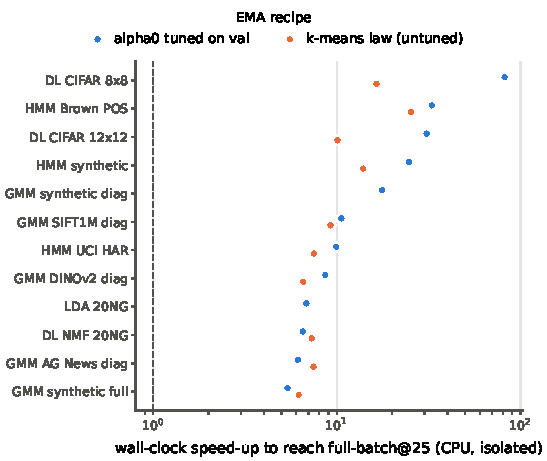
\includegraphics[width=0.75\linewidth]{timing_speedup.pdf}
\caption{Matched-quality wall-clock speed-ups over full-batch EM@25 (log scale).}
\label{fig:timing}
\end{figure}

\subsection{Does the $k$-means law transfer? (C4)}

Applied unchanged, the $k$-means law costs a median validation penalty of $\le 0.2\%$ relative to the swept optimum
on GMM, HMM, dictionary learning and ALS. On HMMs the untuned law reaches Baum--Welch@25 before tuned stepwise EM
(0.95--2.2 vs 1.3--5.7 epochs) but ends slightly above it (e.g.\ Brown 5.215 vs 5.209 nats/token, within one seed
standard deviation).

The law fails on LDA. It predicts $\alpha_0 \approx 0.2$--1, while the swept optimum is 0.005--0.04 (median 0.029).
With the law's rate, held-out perplexity \emph{worsens} with more epochs, and the batch reference is never reached.
The median swept $\aopt$ per family is ALS 0.21, DL 0.26, GMM 0.32, HMM 1.0, LDA 0.029 (Figure~\ref{fig:sweeps}).

\begin{figure}[t]
\centering
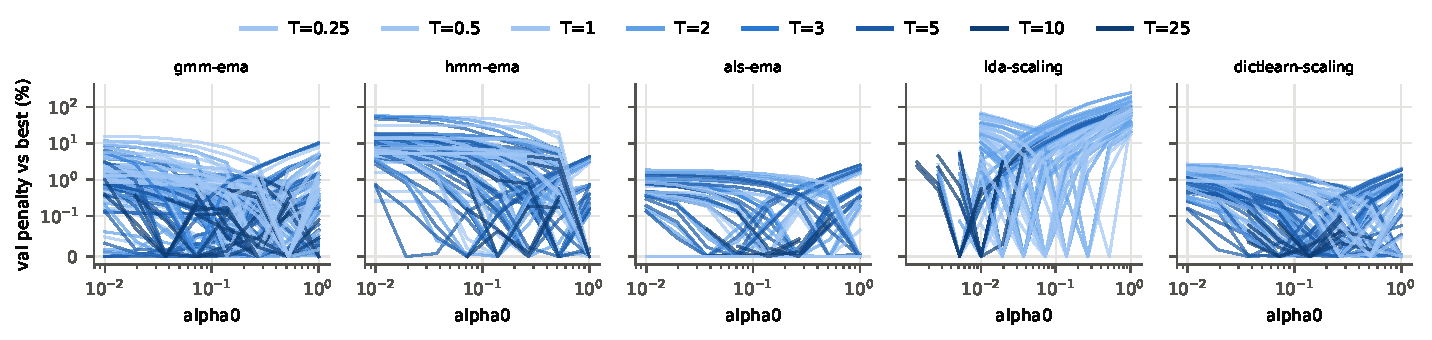
\includegraphics[width=\linewidth]{alpha0_sweeps.pdf}
\caption{Validation penalty against $\alpha_0$ divided by the global law's prediction (dashed line at 1), median over
sweep cells in 0.25-decade bins, grouped by budget. The law is fitted in-sample here; out-of-sample penalties are in
Figure~\ref{fig:penalties}.}
\label{fig:sweeps}
\end{figure}

\subsection{One law across families (C5, C6)}

\paragraph{Pre-registered test (C5).} On 422 swept cells, M1 (log-linear in $n/k$, $B$, $T$ with per-family
intercepts) beats the per-family-constant null M0: leave-one-cell-out median penalty 0.108\% vs 0.319\% (Wilcoxon
$p = 1.05 \times 10^{-18}$); leave-one-family-out median 0.338\% vs 0.440\%. Held-out-family penalties stay large for
LDA (M1 27.7\%) and HMM (4.5\%).

\paragraph{Per-cell coordinates (C6, exploratory).} The law's coordinate $n/k$ counts observations per cluster per
pass. That is the right count for $k$-means and GMMs, but not for models whose statistics are sparse cells:
topic--word counts in LDA and emission counts in HMMs. Counting the observations that reach each statistic cell per
step, a single global law (no per-family constants),
\begin{equation}
  \aopt = 0.419 \cdot \qeff^{0.427} \cdot (n/B)^{-0.282} \cdot T^{-0.326},
\end{equation}
explains $R^2 = 0.66$ of the variance of $\log\aopt$ (vs 0.20 for the same global fit in $n/k$ coordinates). Its
leave-one-family-out median penalty is 0.149\%, and it cuts the LDA held-out penalty from 27.7\% (M1) to 11.6\%. With
per-family constants (Qe1), LOCO is 0.073\% and LDA held-out is 5.3\% (Figures~\ref{fig:penalties}
and~\ref{fig:coords}; all fits in Appendix~\ref{app:law}). The gain is concentrated on LDA: on median
leave-one-family-out penalty the unchanged $k$-means law (0.155\%) is almost as good as Qe0 (0.149\%), and it predicts
HMMs better (0.19\% vs 1.52\%).

The law is not universal. The exponent on $\qeff$ is 0.43, not 1, so the recipe does not hold a fixed number of
observations per cell in its EMA; observations held at the peak rate range from about 7 (LDA) to about 150
(dictionary learning). HMMs want the maximum rate ($\aopt = 1$) despite receiving about one observation per cell per
step.

A natural next feature is the fraction of missing information, which theory links to EM's convergence rate. In an
exploratory test we used the normalised posterior entropy of the latents on held-out data, $h$, as a proxy. It does
not help: adding $\log(1 - h)$ raises $R^2$ only from 0.66 to 0.67 and worsens the leave-one-family-out penalty
(0.149\% $\to$ 0.167\%). The fitted sign is also the opposite of the hypothesis: more missing information goes with a
\emph{larger} $\aopt$, driven by HMMs. LDA's latents are no more uncertain than the HMMs' ($h \approx 0.16$--0.24 vs
0.04--0.47), yet LDA needs an $\alpha_0$ about 30$\times$ smaller. Whatever sets LDA's rate is specific to LDA.

\begin{figure}[t]
\centering
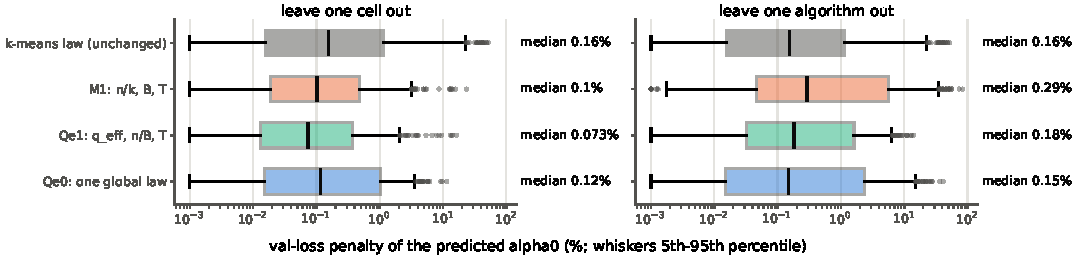
\includegraphics[width=0.85\linewidth]{law_penalties.pdf}
\caption{Validation penalty of the predicted $\alpha_0$ for each law, leave-one-cell-out (left) and
leave-one-family-out (right), over all 422 cells; boxes are quartiles, whiskers the 5th--95th percentiles.}
\label{fig:penalties}
\end{figure}

\begin{figure}[t]
\centering
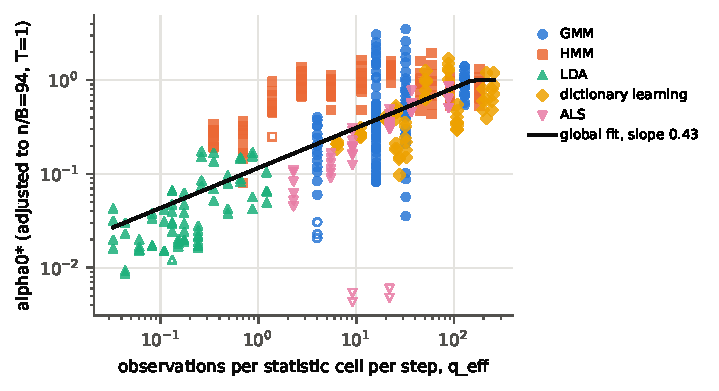
\includegraphics[width=0.75\linewidth]{law_coords.pdf}
\caption{Swept $\aopt$ vs observations per statistic cell per step ($\qeff$), all 422 cells. Each $\aopt$ is moved to a
common $n/B$ (94) and $T = 1$ along the fitted exponents; the line is the single global fit Qe0 (slope 0.43). Hollow =
censored at the grid's lower edge, excluded from the fit. LDA's low rates fall on the same trend as the other families
once cells are counted per statistic; HMMs (squares) sit far above the line at $\aopt \approx 1$.}
\label{fig:coords}
\end{figure}

%======================================================================================================================
\section{Discussion}

\paragraph{What transfers from e-means, and what does not.}
The update and the revival rule transfer as they are. The update was already known to work across families
\citep{liang2009online}. Revival has prior art in online EM \citep{sato2000online,hughes2013memoized} but is absent
from the standard stepwise-EM baselines, and it decides whether online EM works at all on full-covariance mixtures and
LDA. The cosine schedule transfers with a family-dependent benefit: large on HMMs, modest on GMMs and dictionary
learning, none on LDA. The rate law transfers in form but not in coordinates: LDA shows that $n/k$ is the wrong
variable, and the per-cell coordinate is a partial fix.

\paragraph{When is stochastic EM worth it?} Epoch gains are largest where the batch E-step is expensive and the
statistics are dense relative to the batch: HMMs, dictionary learning, diagonal GMMs. They are smallest where the
batch method is already near convergence after a few passes (ALS ML-1M) or where the statistics are sparse (LDA
NYTimes).

\paragraph{Limitations.}
\begin{enumerate}[nosep]
  \item \emph{Datasets} are narrower than planned: MovieLens 1M/10M instead of 25M/Netflix; Brown instead of Penn
        Treebank; no PubMed/Wikipedia LDA; no audio dictionary learning.
  \item \emph{Reference.} The reference is batch EM at 25 iterations, not converged batch EM.
  \item \emph{Long budgets} use a frozen 3--4-point local search for all methods.
  \item \emph{Wall-clock} covers matches within 5 epochs only (12 of the 17 configurations the recipe matches), on one
        CPU.
  \item \emph{GPU kernels.} We did not combine either side with fused GPU kernels (Flash-KMeans / Flash-GMM).
  \item \emph{Post-hoc analyses.} The revival-equipped baseline and the per-cell law were added after seeing results.
  \item \emph{Operational repairs}, all disclosed and none changing a method: an LDA E-step aliasing bug (all LDA
        re-run), a scheduler bug (73 jobs re-run), 17 HMM jobs re-run after GPU errors, one ALS cell filled, and
        three missing SIFT1M full-covariance reference seeds filled (Appendix~\ref{app:repairs}).
  \item \emph{Revival and rare groups.} Our revival rule judges a unit by its mass alone, as e-means does, so it can
        delete a small component that covers a rare, isolated group \citep{weiss2026small}. In a GMM ablation
        (Appendix~\ref{app:rare}; exploratory, 3 seeds) this costs likelihood on rare classes (Covertype: rare-class NLL
        $-41.4$ vs $-43.2$ without revival at 5 epochs; KDD Cup 99: worse than no revival overall at 5 epochs). A
        distance-aware variant recovers most of the loss, and on our benchmark data the two rules give identical
        results. Deployments with rare, isolated groups should use the distance-aware rule.
\end{enumerate}

%======================================================================================================================
\section{Conclusion}

Within the scope we tested, the e-means recipe is a recipe for stochastic-approximation EM in general, not only for
$k$-means. Revival and a budget-aware cosine schedule let a stepwise EM update reach the batch objective in a few
epochs across mixtures, HMMs, dictionary learning, topic models and matrix factorisation. The $k$-means rate law
carries over to four of five families, and a law in observations-per-statistic coordinates comes closer to one rule
for all five. LDA is the exception throughout: there, a well-tuned inverse-time schedule with revival is as good, and
the optimal rate is an order of magnitude lower than the law predicts. These are the cases a predictive theory of
stochastic EM step sizes will have to explain.

\paragraph{Reproducibility.} Code, job files and every result record (one JSONL line per run, 44{,}197 runs) are
provided as anonymised supplementary material. Verdict tables, figures and law fits are regenerated from the records
without re-running any experiment; the full protocol is about 575 job-hours on one desktop. Hypotheses and kill
criteria were frozen before the runs, and amendments are logged.

\bibliography{references}
\bibliographystyle{\bibstylename}

%======================================================================================================================
\appendix

\section{Datasets}\label{app:data}
SIFT1M \citep{jegou2011pq} via ANN-Benchmarks \citep{aumuller2020ann}; DINOv2-S features \citep{oquab2024dinov2} of
CIFAR-100 \citep{krizhevsky2009learning}; all-MiniLM-L6-v2 embeddings \citep{reimers2019sbert,wang2020minilm} of AG
News \citep{zhang2015character}; 20 Newsgroups \citep{lang1995newsweeder}; Enron and NYTimes from the UCI
bag-of-words collection \citep{newman2008bow}; MovieLens \citep{harper2015movielens}; the Brown corpus
\citep{francis1979brown} with the universal tagset \citep{petrov2012universal}; UCI HAR \citep{anguita2013har}. ALS
follows ALS-WR \citep{zhou2008netflix}. Embeddings are reduced to 64 dimensions by PCA fitted on the training split.
Datasets are not redistributed; the released download script fetches each from its provider. Licences and required
citations are listed in the supplementary material.

\section{Hyperparameter grids}\label{app:grids}
\begin{itemize}[nosep]
  \item \textbf{Recipe $\alpha_0$ grid (swept).} Eight log-spaced values on $[0.01, 1]$: $\{0.01, 0.0193, 0.0373,
        0.0720, 0.1389, 0.2683, 0.5179, 1\}$. For LDA, where a third of the cells chose 0.01, the grid continues
        downwards with the same spacing by five values ($0.00518, 0.00268, 0.00139, 0.00072, 0.00037$).
  \item \textbf{Tuned stepwise / online EM.} $\alpha_t = (\tau_0 + t)^{-\kappa}$ with $\kappa \in \{0.5, 0.6, 0.7,
        0.8, 0.9, 1.0\}$; $\tau_0 \in \{2, 10, 100\}$ for HMM, LDA, dictionary learning and ALS (18 settings) and
        $\tau_0 \in \{1, 10, 100, 1000\}$ for GMMs (24 settings). The same grid is used with and without revival.
        The online-LDA library default is $\tau_0 = 1024$, $\kappa = 0.7$.
  \item \textbf{Batch sizes} for the headline curves: GMM 1024; HMM, LDA and dictionary learning 256; ALS 256
        (ML-1M) and 2048 (ML-10M). The \emph{law} method uses the e-means batch law instead.
  \item \textbf{Long budgets ($T = 10, 25$).} Before any long run, a plan file froze, per configuration, the four
        $\alpha_0$ grid values around the recipe's $T = 5$ optimum (two below, one above) and the three best
        $(\tau_0, \kappa)$ settings of the tuned baseline at $T = 5$. An optimum at the edge of a restricted grid is
        treated as censored in the law fits.
  \item \textbf{Law-fitting cells.} Besides the headline cells, each family sweeps $\alpha_0$ over sub-sampled
        problems: GMM $n \in \{n/4, n/2, n\}$, $B \in \{256, 2048\}$, $T \in \{1, 2, 5\}$; HMM $n \in \{n/4, n/2,
        n\}$, $B \in \{64, 512\}$, $T \in \{1, 2, 5\}$; LDA $n \in \{n/4, n\}$, $B \in \{64, 512\}$, $T \in \{1,
        2\}$; dictionary learning $n \in \{n/4, n\}$, $B \in \{64, 512\}$, $T \in \{1, 2, 5\}$; ALS $B \in
        \{B_h/4, B_h, 4B_h\}$, $T \in \{1, 2, 5\}$. Together with the headline cells this gives the 422 cells used
        in Section~5.5.
  \item \textbf{Fixed model settings.} ALS regularisation $\lambda$ is chosen once from $\{0.01, 0.03, 0.05, 0.1,
        0.2\}$ on validation (seed 0) and shared by every method. The cosine floor is $\varepsilon = 0.1$ and
        revival runs every 5 batches with threshold 0.1 for every family that uses it.
\end{itemize}

\section{Deviations and repairs}\label{app:repairs}
\begin{itemize}[nosep]
  \item \textbf{LDA E-step aliasing bug.} In the parallel (numba) LDA E-step a hoisted allocation made two
        per-document buffers alias, so every document stopped after 2 E-step iterations instead of iterating to
        tolerance. It was found because a GPU port disagreed with the CPU path. After the fix (with a regression test)
        every LDA stage was re-run; earlier LDA records are archived and none is used.
  \item \textbf{Scheduler adoption bug.} On restart the queue adopted a running process under 2--3 job ids that
        differed only in an environment variable, and marked all of them done when it exited. This affected 73 jobs
        (GMM SIFT1M diag and full, DINOv2 full, synthetic full; dictionary learning CIFAR $8{\times}8$ seed 0); they
        and 10 dependent jobs were re-queued, and stale records were moved aside.
  \item \textbf{HMM GPU errors.} 17 HMM jobs failed with GPU errors and were re-run.
  \item \textbf{ALS.} One missing ALS cell was filled.
  \item \textbf{SIFT1M full-covariance reference.} The batch reference for this configuration initially had seeds
        3--4 only; seeds 0--2 were run later with the same command. With 5 seeds the reference moves from 40.67 to
        40.69 nats, and epochs-to-match change from 7.86 to 7.24 (swept), 16.1 to 14.8 (law) and 11.8 to 10.4
        (tuned + revival). No count or test in the paper changes.
\end{itemize}

\section{Law fits}\label{app:law}
\begin{table}[h]
\centering\small
\caption{Law comparison on 422 swept cells (15 censored at the grid's lower edge). Penalties are median relative
validation losses; LDA held out gives the penalty and (predicted / best $\alpha_0$). The pre-registered test in the
main text (M1 vs M0) uses the pre-registered fitting script, whose cross-validation gives M1 LOCO 0.108\% and LOAO
0.338\%; the numbers below come from the exploratory refit, which reproduces M1 within 0.05 points.}
\label{tab:laws}
\begin{tabular}{p{4.6cm}cccp{3.0cm}p{1.6cm}}
\toprule
model & LOCO & LOAO & HMM held out & LDA held out & $R^2$, one global law \\
\midrule
$k$-means law (unchanged) & 0.155\% & 0.155\% & 0.19\% & 16.3\% (0.187 / 0.037) & --- \\
M1: $n/k$, $B$, $T$ (+ per-family constant) & 0.103\% & 0.290\% & 4.54\% & 27.7\% (0.27 / 0.037) & 0.20 \\
Q1: $q$, $n/B$, $T$ (+ per-family constant) & 0.076\% & 0.225\% & 4.79\% & 6.4\% (0.088 / 0.037) & 0.50 \\
Q0: one global law in $q$ & 0.193\% & 0.249\% & 4.54\% & 29.9\% (0.309 / 0.037) & 0.50 \\
Qe1: $\qeff$, $n/B$, $T$ (+ per-family constant) & 0.073\% & 0.183\% & 1.81\% & 5.3\% (0.067 / 0.037) & 0.66 \\
\textbf{Qe0: one global law in $\qeff$} & 0.116\% & \textbf{0.149\%} & 1.52\% & 11.6\% (0.134 / 0.037) & \textbf{0.659} \\
\bottomrule
\end{tabular}
\end{table}
Every coordinate law predicts HMMs worse than the unchanged $k$-means law (1.5--4.8\% vs 0.19\%), and the unchanged
$k$-means law's leave-one-family-out median (0.155\%) is close to Qe0's (0.149\%). The per-cell coordinate's gain is
concentrated on LDA.

\section{Revival on rare groups}\label{app:rare}
\textbf{Question.} \citet{weiss2026small} report, for $k$-means, that count-based revival deletes clusters covering
rare isolated groups. Does the recipe's rule do the same in EM?

\textbf{Setup.} GMM recipe (cosine EMA, $B = 1024$, $\varepsilon = 0.1$) with three revival modes: \emph{off};
\emph{count} (the recipe's rule); \emph{dist}, Weiss's rule adapted to GMMs, where a count-flagged component is
re-seeded only if $\min_i \|\mu_j - \mu_i\|^2 \le 4\,\mathrm{MSE}$, with $\mathrm{MSE} = \sum_j w_j \operatorname{tr}
\Sigma_j$, or if it has had fewer than 0.5 points of batch mass for 2 epochs. $\alpha_0$ is selected on validation
NLL from $\{0.072, 0.139, 0.268, 0.518, 1.0\}$ per (dataset, method, $T$); seeds 0--2; $T \in \{2, 5\}$. Tail NLL is
the mean test NLL on rare groups (the synthetic small clusters, or labelled classes with $< 2\%$ of training points).
Data: a synthetic far-groups mixture ($d = 16$; 30 large clusters and 4 at radius 30 with 0.2\% mass each; diagonal
and full, $k = 34$); Statlog Shuttle; KDD Cup 99 (10\%, 38 numeric columns); Covertype; SIFT1M-PCA64 as a control;
real data standardised, $k = 64$, diagonal. KDD Cup 99 and Covertype use a covariance floor of 0.01 (standardised
units) instead of the recipe's relative floor, because components otherwise collapse onto binary columns.

\begin{table}[h]
\centering\small
\caption{Test NLL (seed means, 3 seeds) at the validation-selected $\alpha_0$; tail NLL in brackets; lower is
better.}\label{tab:rare}
\begin{tabular}{llccc}
\toprule
dataset & $T$ & off & count (recipe) & dist (Weiss) \\
\midrule
SIFT1M control & 2 & 60.02 & 59.30 & 59.30 (identical) \\
SIFT1M control & 5 & 59.92 & 59.21 & 59.21 (identical) \\
synthetic diag & 2 & 27.36 [61.5] & 27.00 [53.8] & 26.98 [53.8] \\
synthetic diag & 5 & 27.40 [62.0] & \best{26.32} [53.9] & 26.48 [53.9] \\
synthetic full & 2 & 26.48 [34.3] & 26.56 [36.3] & 26.50 [34.7] \\
synthetic full & 5 & 26.47 [34.4] & 26.54 [36.3] & 26.49 [34.8] \\
Shuttle & 2 & $-8.35$ [19.7] & $-11.11$ [16.8] & $-10.99$ [21.8] \\
Shuttle & 5 & $-9.18$ [16.8] & $-12.14$ [19.5] & $-12.11$ [14.9] \\
KDD Cup 99 & 2 & $-45.82$ [2.4] & $-46.58$ [5.2] & \best{$-47.07$} [\best{$-12.0$}] \\
KDD Cup 99 & 5 & \best{$-47.41$} [\best{$-24.9$}] & $-46.27$ [15.4] & $-46.93$ [$-6.9$] \\
Covertype & 2 & $-45.29$ [$-43.25$] & $-45.25$ [$-41.59$] & \best{$-45.57$} [$-43.05$] \\
Covertype & 5 & $-45.24$ [$-43.25$] & $-45.20$ [$-41.44$] & \best{$-45.47$} [$-42.29$] \\
\bottomrule
\end{tabular}
\end{table}

Where rare isolated groups exist, count-based revival costs tail likelihood (Covertype 1.7--1.8 nats on rare classes;
KDD Cup 99 by 3--40 nats; synthetic full covariance 2 nats), and on KDD Cup 99 at $T = 5$ it is worse overall than no
revival. The distance-aware rule removes most of that cost while keeping revival's gains where they exist (Shuttle
$-12.1$ vs $-9.2$ without revival). On SIFT1M the distance test never fires and results are identical, so the main
results are unaffected. Tail sets are small (Shuttle 39 points, KDD Cup 99 367, Covertype 431) and KDD Cup 99 tail
variance is large; only GMMs were tested.

\section{Compute}\label{app:compute}
About 575 job-hours for the main protocol plus 273 ablation jobs, on one desktop (Ryzen 9 9900X, RTX 5090); software
versions are pinned in the released lock file.

\end{document}
